% --------------------------------------------------------------
% This is all preamble stuff that you don't have to worry about.
% Head down to where it says "Start here"
% --------------------------------------------------------------
 
\documentclass[12pt]{article}
 
\usepackage[margin=1.5cm,top=1cm]{geometry} 
\usepackage[utf8]{inputenc}
\usepackage[T1]{fontenc}
\usepackage[dvips]{graphicx}
\usepackage{xcolor}
\usepackage{times}
\usepackage{amsmath,amsthm,amssymb}
\usepackage{dsfont}
\usepackage{slashed}
\usepackage{mathtools}
\usepackage[shortlabels]{enumitem}
\usepackage{tikz}
\usepackage{tikz-3dplot}
\usetikzlibrary{decorations.pathmorphing}
\usetikzlibrary{decorations.markings}
\usetikzlibrary{arrows.meta}
\usetikzlibrary{shapes.symbols}
\usetikzlibrary{calc}



\newenvironment{problem}[2][Problem]{\begin{trivlist}
\item[\hskip \labelsep {\bfseries #1}\hskip \labelsep {\bfseries #2.}]}{\end{trivlist}}

\begin{document}
 
% --------------------------------------------------------------
%                         Start here
% --------------------------------------------------------------
 
\title{Homework 1 Classical Mechanics\\Deadline August 21, 2023.}
\date{}
 
\maketitle



\begin{problem}{1}
Determine the Lagrangian and the equations of motion of a bob of mass $m$ suspended from an inextensible massless rod of length $l$ in terms of the polar and azimuthal angles, with gravity acting downwards.
\begin{center}
\tdplotsetmaincoords{60}{110}
%
\pgfmathsetmacro{\rvec}{.8}
\pgfmathsetmacro{\thetavec}{120}
\pgfmathsetmacro{\phivec}{60}
%
\begin{tikzpicture}[scale=5,tdplot_main_coords]
    \coordinate (O) at (0,0,0);
    \draw[thick,->,dashed] (0,0,0) -- (1,0,0) node[anchor=north east]{$x$};
    \draw[thick,->,dashed] (0,0,0) -- (0,1,0) node[anchor=north west]{$y$};
\draw[thick,->,dashed] (0,0,0) -- (0,0,1) node[anchor=south]{$z$};
    \tdplotsetcoord{P}{0.8}{\thetavec}{\phivec}
    \tdplotsetcoord{Q}{0.4}{\thetavec}{\phivec}
    \draw[thick,-,color=blue] (O) -- (P) node[above right,color=black] {$m$};
    \draw[->] (0.5,0,0.8) -- node[left] {$g$}(0.5,0,0.4) ;
	\node at (P)[circle,fill,inner sep=3pt] {};
	\draw (Q) node[anchor=north east]{$ l $}; 
    \draw[dashed, color=blue] (O) -- (Pxy);
    \draw[dashed, color=blue] (P) -- (Pxy);
    \tdplotdrawarc[color=red]{(O)}{0.2}{0}{\phivec}{anchor=north,color=black}{$\phi$}
    \tdplotsetthetaplanecoords{\phivec}
    \tdplotdrawarc[tdplot_rotated_coords, color=red]{(0,0,0)}{0.5}{0}%
        {\thetavec}{anchor=south west,color=black}{$\theta$}
\end{tikzpicture}
\end{center}
 
\end{problem}
\newpage

\begin{problem}{2}
A bead of mass $m$ slides on a massive frictionless hoop of radius $a$. The hoop is rotating at a constant angular speed $\omega$ about a vertical axis under a constant gravitational acceleration.  Determine the Lagrangian and the equation of motion.
\begin{center}
\begin{tikzpicture}[important line/.style={thick,blue},scale=1.5]
\newcommand{\AxisRotator}[1][rotate=0]{%
    \tikz \draw[x=.5em,y=1.25em,line width=.2ex,-stealth,#1] (0,0) arc (-150:150:1 and 1);%
}
\draw [important line,fill=white,opacity=1] (0,0) circle (1.5cm and 2cm);%top of cone
\draw[thick,->,dashed] (0,-2.5) -- (0,3.5)node[anchor=south]{$z$}; %axis
\draw[thick,->,dashed] (-2,0.7) -- (2,-0.7); %axis
\draw[-] (0,0) -- (1,-1.5); %axis
\draw (0.3,-1) node{$ \theta $}; % theta
\draw (0.7,-0.5) node{$ a $}; 
\draw[->] (-2,2) -- node[left] {$g$}(-2,1) ;
\node at (1,-1.5)[circle,fill,inner sep=3pt] {};
\node at (1.2,-1.75)[]{$m$};
\node at (0.7,2.5)[]{$\omega$};
\draw (0,2.5) node {\AxisRotator[rotate=-90]}; 
\draw[red] (0,-0.75) arc (-90:-57:0.75);
\end{tikzpicture}
\end{center}
\end{problem}

\begin{problem}{3}
Find the Lagrangian and equations of motion for a point mass $m$ connected to one end of a massless spring of rest length $l_0$ and spring constant $k$, whose other end is fixed, assuming that the motion takes place on the plane and that gravity pulls downwards. 
\begin{center}
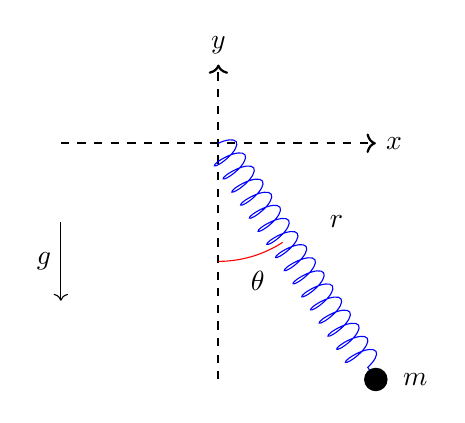
\begin{tikzpicture}
        \draw[thick,->,dashed] (-2,0) -- (2,0) node[right] {$x$};
        \draw[thick,->,dashed] (0,-3) -- (0,1) node[above] {$y$};
        \draw[->] (-2,-1) -- node[left] {$g$}(-2,-2) ;
        \draw[decoration={aspect=0.3, segment length=2mm, amplitude=2mm,coil},decorate,color=blue] (0,0) -- (2,-3); 
\node at (2,-3)[circle,fill,inner sep=3pt]{};
\node at (2.5,-3)[]{$m$};
\draw[red] (0,-1.5) arc (-90:-57:1.5);
\draw (0.5,-1.75) node{$ \theta $};
\draw (1.5,-1) node{$ r $};
\end{tikzpicture}
\end{center}
\end{problem}

Solucion
\begin{problem}{4}
Consider a planar pendulum of mass $m$ connected to to a hinge by a massless rod of time–dependent length $s(t)$, moving under a constant gravitational field. Determine the Lagrangian and the Euler-Lagrange equations. 
\begin{center}
\begin{tikzpicture}
        \draw[thick,->,dashed] (-2,0) -- (2,0) node[right] {$x$};
        \draw[thick,->,dashed] (0,-3) -- (0,1) node[above] {$y$};
        \draw[->] (-2,-1) -- node[left] {$g$}(-2,-2) ;
        \draw[thick,-,color=blue] (0,0) -- (2,-3); 
\node at (2,-3)[circle,fill,inner sep=3pt]{};
\node at (2.5,-3)[]{$m$};
\draw[red] (0,-1.5) arc (-90:-57:1.5);
\draw (0.5,-1.75) node{$ \theta $};
\draw (1.5,-1) node{$ s(t) $};
\end{tikzpicture}
\end{center}
\end{problem}

\begin{problem}{5} 
A uniform hoop of mass $m$ and radius $r$ rolls without slipping on a fixed cylinder of radius $R$. The only external force is that of gravity. If the smaller cylinder starts rolling from rest on top of the bigger cylinder, use the method of Lagrange mulipliers to find the point at which the hoop falls off the cylinder.
\begin{center}
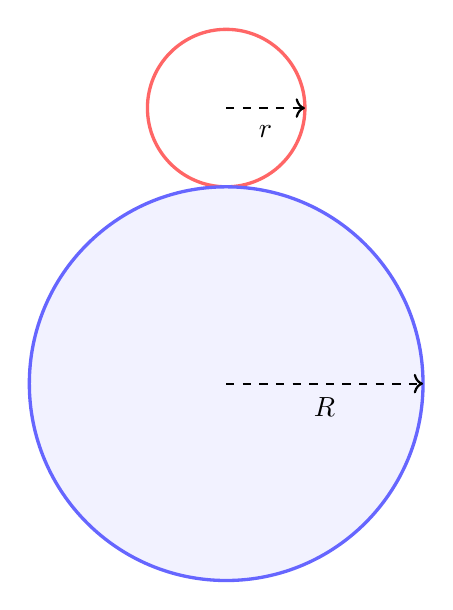
\begin{tikzpicture}
\filldraw[color=red!60, fill=white, very thick](0,1) circle (1);
\draw[thick,->,dashed] (0,1) -- (1,1);
\draw (0.5,0.7) node{$ r$};
\filldraw[color=blue!60, fill=blue!5, very thick](0,-2.5) circle (2.5);
\draw[thick,->,dashed] (0,-2.5) -- (2.5,-2.5);
\draw (1.25,-2.8) node{$R$};
\end{tikzpicture}
\end{center}
\end{problem}

 
\end{document}